% anhang.tex
\chapter{Weitere Informationen}
\section{Alternative Eingabedaten} \label{alternative}
Im Folgenden sind die vollständigen Laufzeitmessungen für die Eingabedaten, sources, english, dna und xml, aufgeführt. Während die absoluten Werte
der Laufzeit für die verschiedenen Eingabedaten variieren, zeigen die Kurven der Laufzeitmessungen eine ähnliche Tendenz.
\begin{figure} [H]
    \centering
    \caption{Laufzeitmessung von LZ77, Approx.LZ77 und Approx.LZ77Par(16 Threads) auf verschiedenen Präfixen von sources. Als Vergleichsmaß wurde 
    die lineare Regression der Kurven gestrichelt eingezeichnet.}
    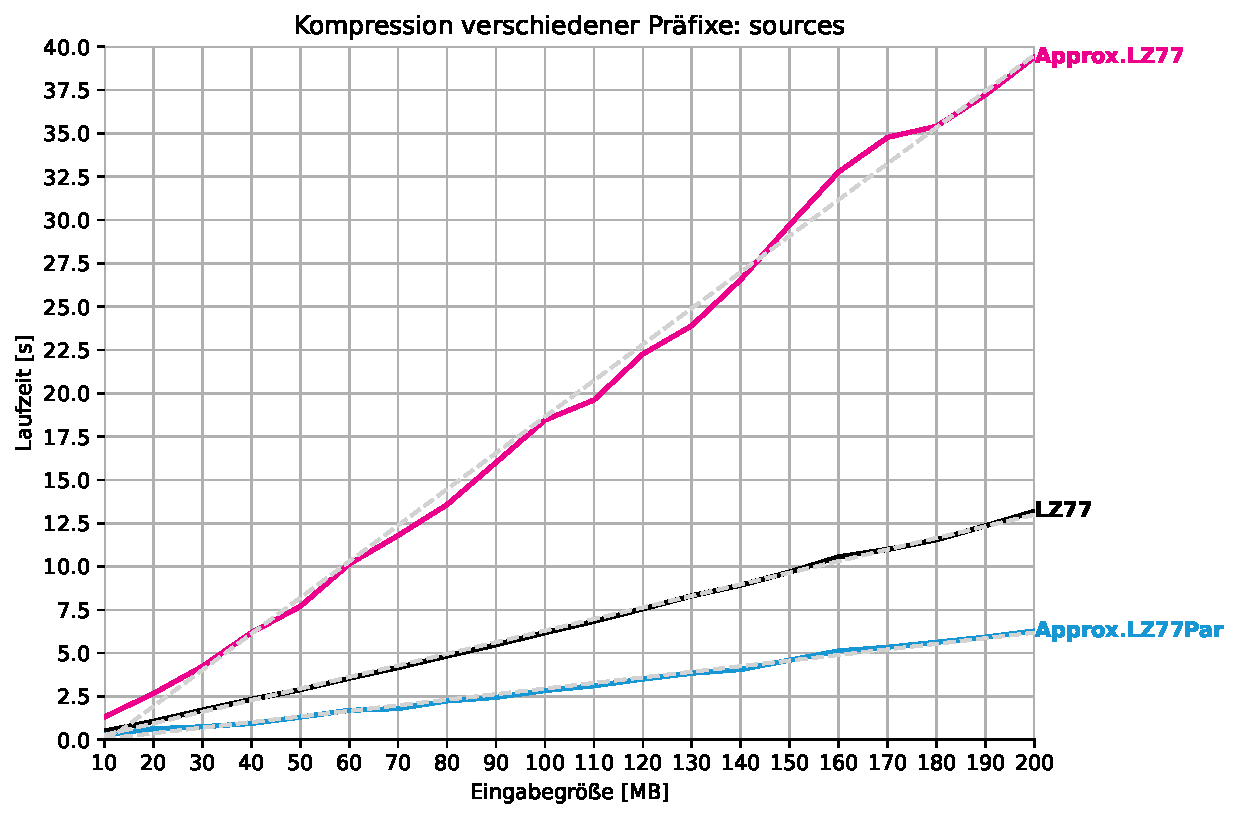
\includegraphics[scale=0.65]{Images/progressive_sources.pdf}
\end{figure}

\begin{figure}[H]
    \centering
    \caption{Laufzeitmessung von Approx.LZ77Par mit verschiedener Anzahl an Threads für sources}
    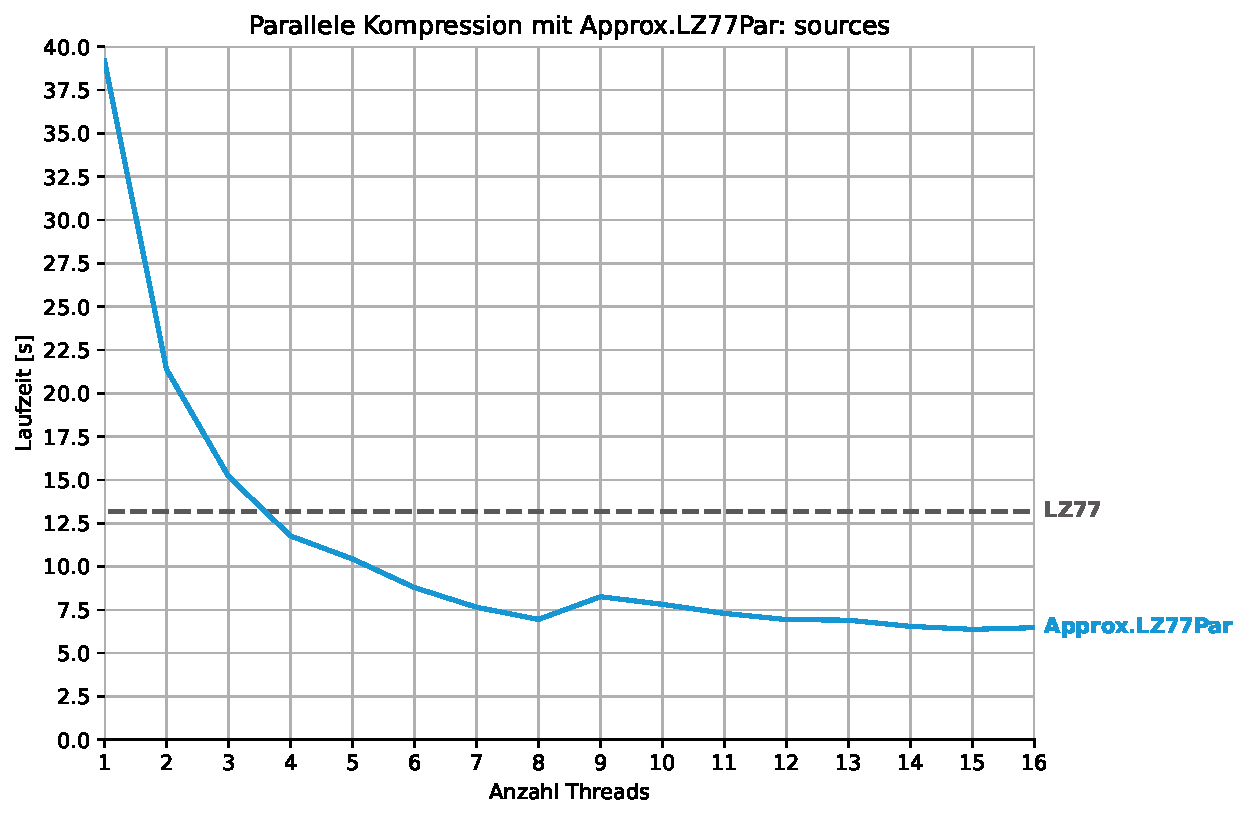
\includegraphics[scale=0.65]{Images/progressive_speedup_sources.pdf}
\end{figure}

\begin{figure}[H]
    \centering
    \caption{Laufzeitmessung von LZ77, Approx.LZ77 und Approx.LZ77Par(16 Threads) auf verschiedenen Präfixen von english. Als Vergleichsmaß wurde 
    die lineare Regression der Kurven gestrichelt eingezeichnet.}
    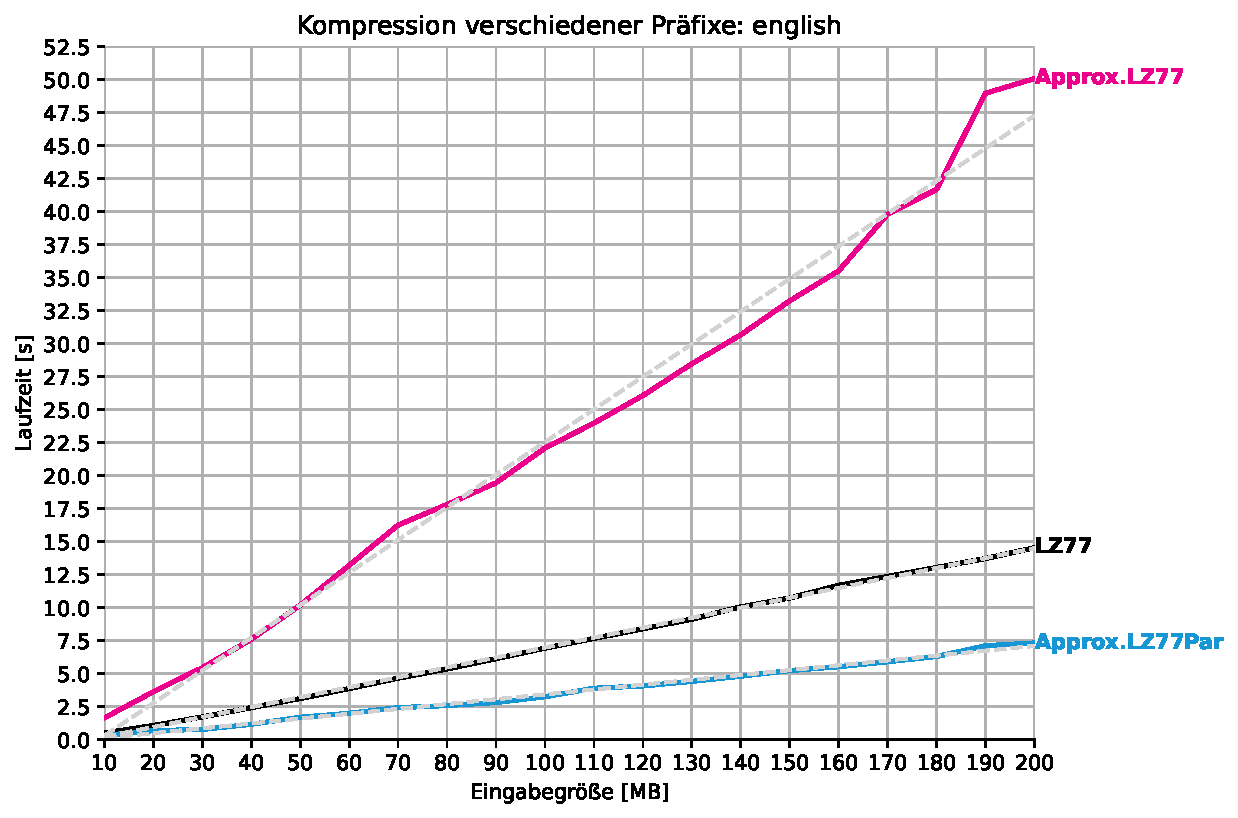
\includegraphics[scale=0.65]{Images/progressive_english.pdf}
\end{figure}

\begin{figure}[H]
    \centering
    \caption{Laufzeitmessung von Approx.LZ77Par mit verschiedener Anzahl an Threads für english}
    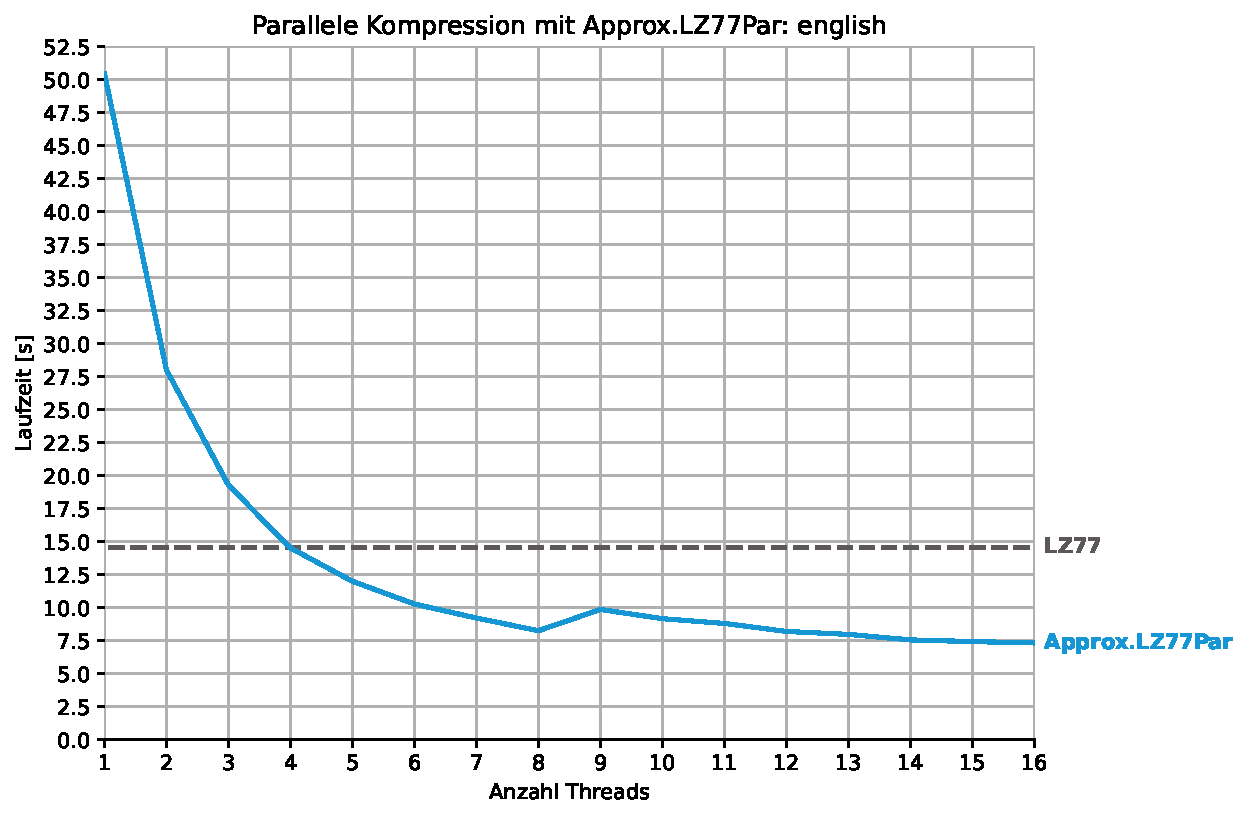
\includegraphics[scale=0.65]{Images/progressive_speedup_english.pdf}
\end{figure}

\begin{figure}[H]
    \centering
    \caption{Laufzeitmessung von LZ77, Approx.LZ77 und Approx.LZ77Par(16 Threads) auf verschiedenen Präfixen von dna. Als Vergleichsmaß wurde 
    die lineare Regression der Kurven gestrichelt eingezeichnet.}
    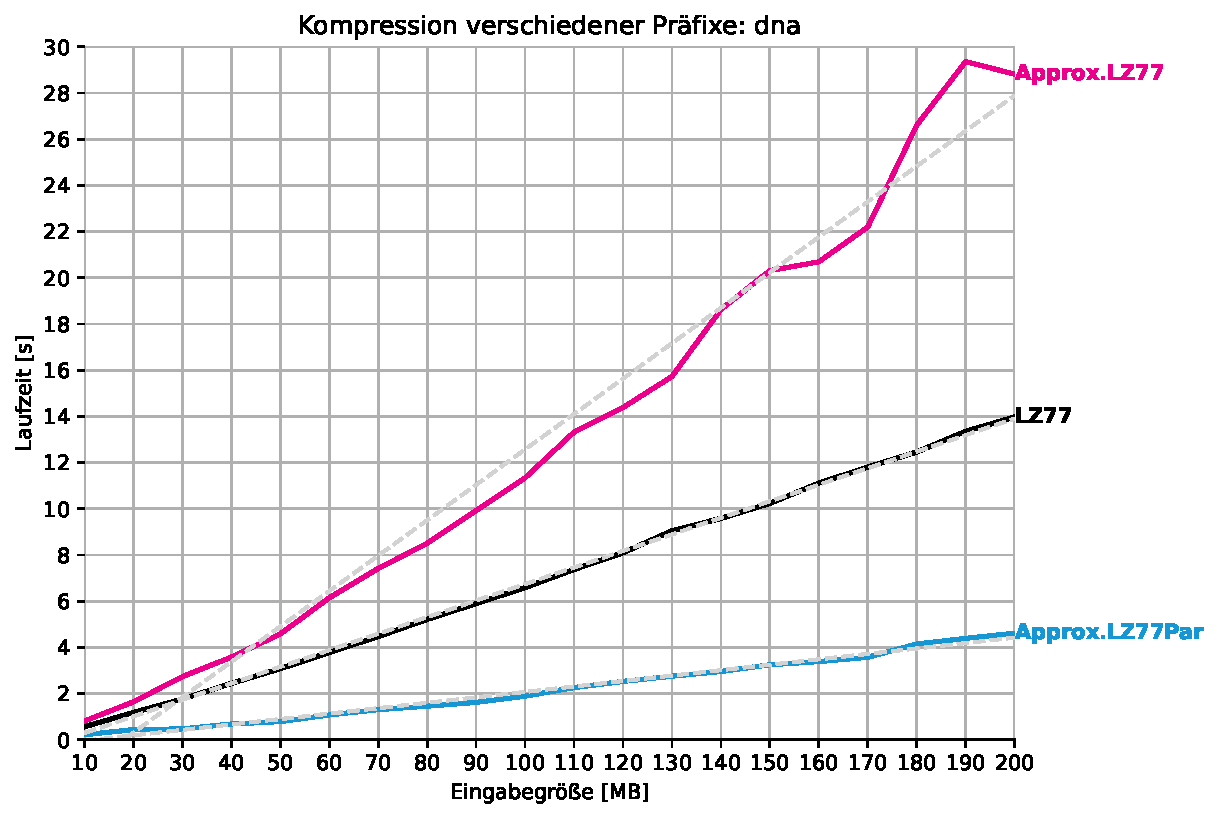
\includegraphics[scale=0.65]{Images/progressive_dna.pdf}
\end{figure}

\begin{figure}[H]
    \centering
    \caption{Laufzeitmessung von Approx.LZ77Par mit verschiedener Anzahl an Threads für dna}
    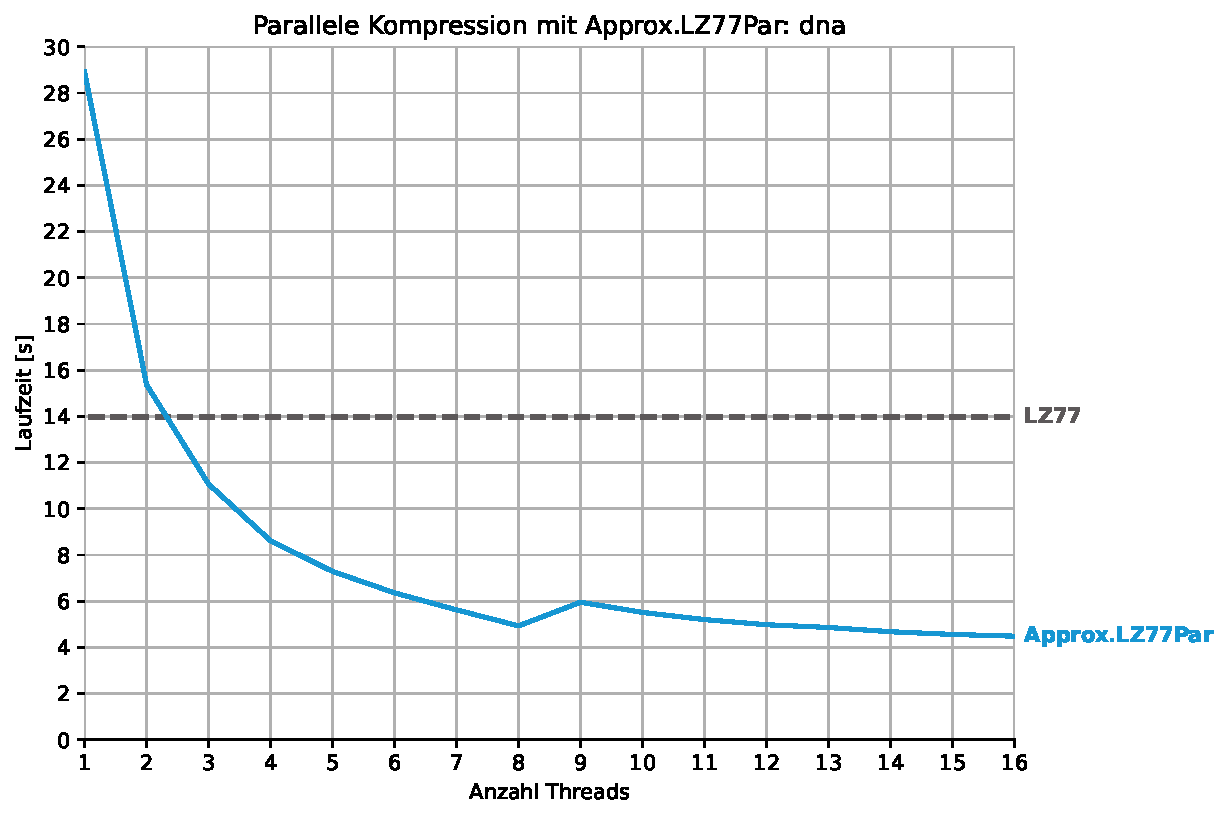
\includegraphics[scale=0.65]{Images/progressive_speedup_dna.pdf}
\end{figure}

\begin{figure}[H]
    \centering
    \caption{Laufzeitmessung von LZ77, Approx.LZ77 und Approx.LZ77Par(16 Threads) auf verschiedenen Präfixen von xml. Als Vergleichsmaß wurde 
    die lineare Regression der Kurven gestrichelt eingezeichnet.}
    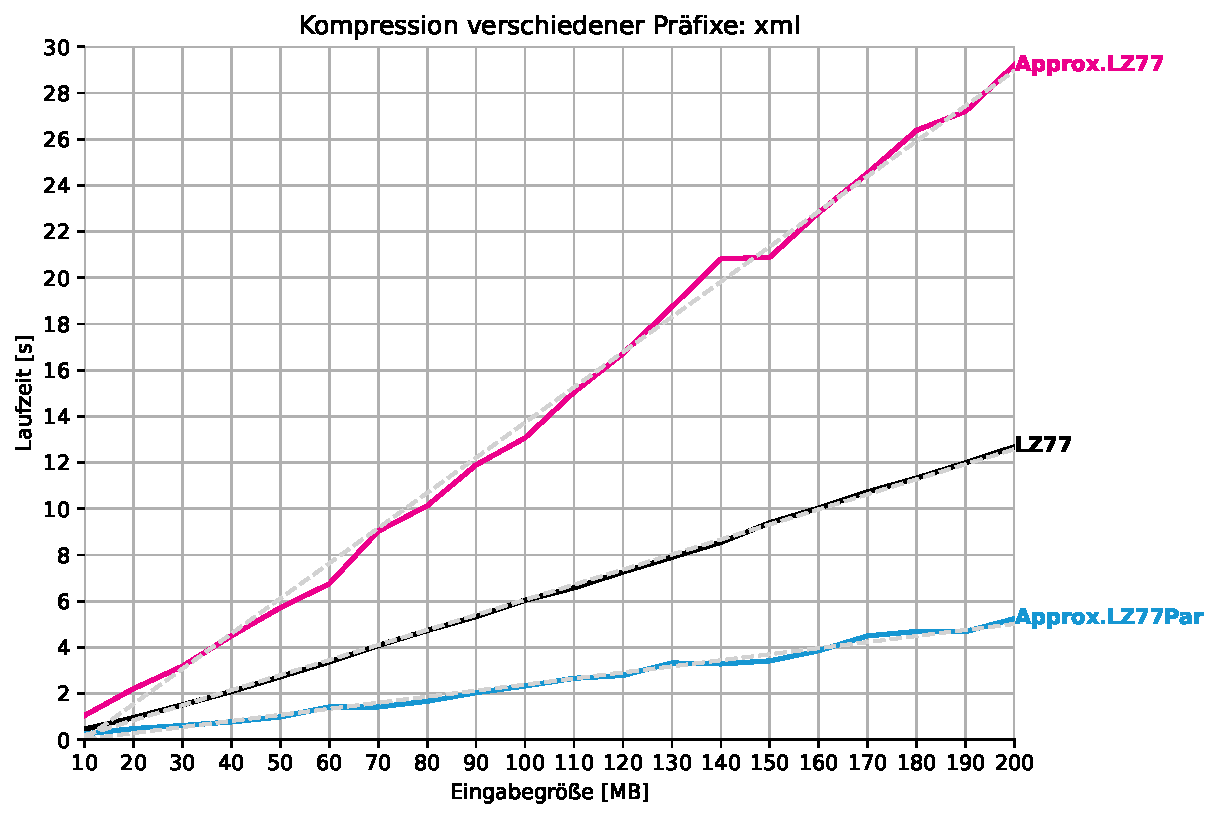
\includegraphics[scale=0.65]{Images/progressive_xml.pdf}
\end{figure}

\begin{figure}[H]
    \centering
    \caption{Laufzeitmessung von Approx.LZ77Par mit verschiedener Anzahl an Threads für xml}
    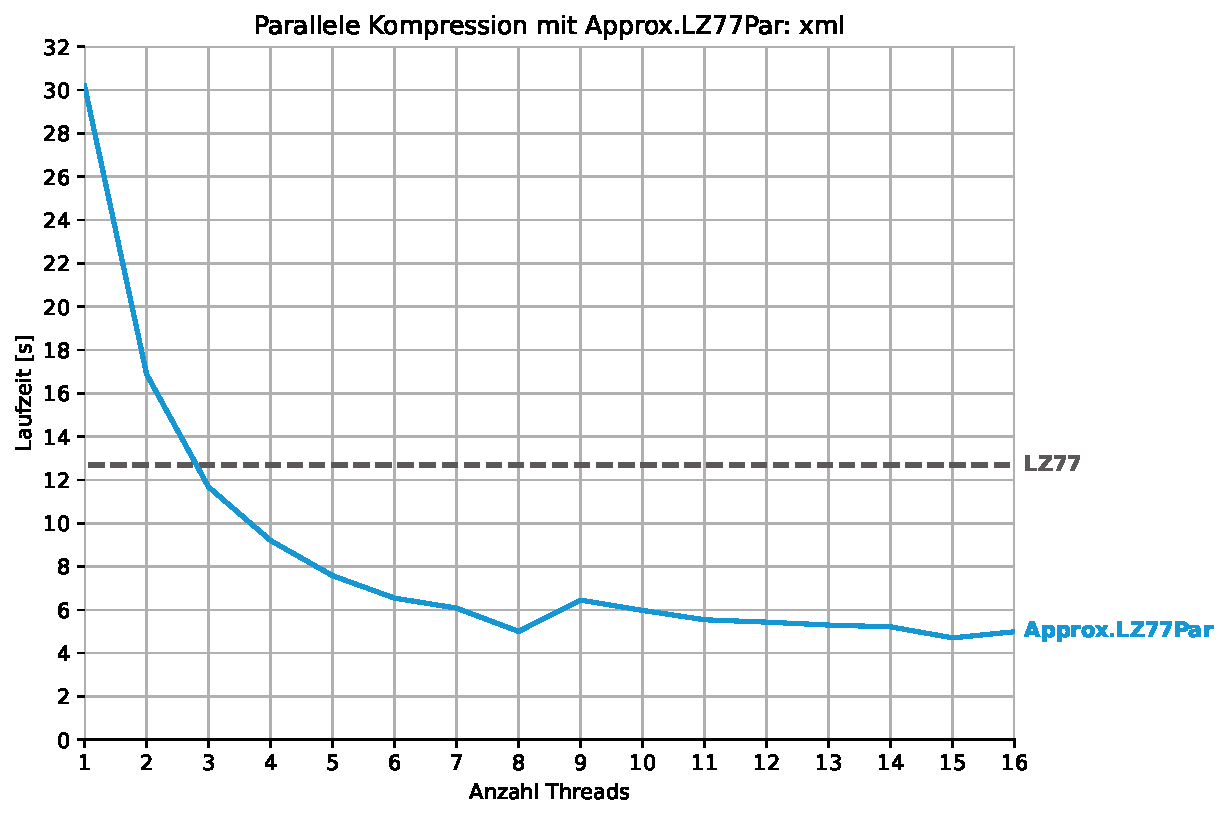
\includegraphics[scale=0.65]{Images/progressive_speedup_xml.pdf}
\end{figure}
\pagebreak
\section{Alternative Testumgebung}
Für die folgenden Messwerte wurden die Algorithmen auf einem Rechner mit einem AMD EYPC 7452 32-Core Prozessor mit 128 nutzbaren Threads ausgeführt.
Die Einstellungen der Algorithmen, die in \ref{settings} etabliert wurden, wurden beibehalten.

\begin{table}[ht]
    \centering
    \caption{Messwerte der Algorithmen auf verschiedenen Eingabedateien}
    \begin{tabular} { |c|c|c|c|c|c| }
        \hline
        \textbf{Eingabe} & \textbf{Algorithmus} & \textbf{Laufzeit[s]} & \textbf{Speicher} & \textbf{FR} & \textbf{CR*} \\
        \hline
        & LZ77 & 30.65 & 14.88 & 9.95\% & 70.92\% \\
        proteins & Approx.LZ77 & 64.46 & 9.94 & 15.34\% & 63.95\% \\
        & Approx.LZ77Par & 4.75 & 9.20 & 15.34\% & 63.95\% \\
        \hline
        & LZ77 & 28.38 & 13.44 & 5.50\% & 39.20\% \\
        sources & Approx.LZ77 & 62.35 & 6.42 & 10.05\% & 40.14\% \\
        & Approx.LZ77Par & 3.86 & 5.51 & 10.05\% & 40.14\% \\
        \hline
        & LZ77 & 33.59 & 13.44 & 6.66\% & 47.45\% \\
        english & Approx.LZ77 & 81.21 & 7.06 & 10.42\% & 43.39\% \\
        & Approx.LZ77Par & 4.30 & 5.95 & 10.42\% & 43.39\% \\
        \hline
        & LZ77 & 28.66 & 13.44 & 6.66\% & 47.46\% \\
        dna & Approx.LZ77 & 46.06 & 8.38 & 10.71\% & 45.53\% \\
        & Approx.LZ77Par & 3.52 & 6.13 & 10.71\% & 45.53\% \\
        \hline
        & LZ77 & 27.89 & 12.72 & 3.35\% & 23.89\% \\
        xml & Approx.LZ77 & 49.88 & 3.46 & 6.62\% & 26.78\% \\
        & Approx.LZ77Par & 2.91 & 3.28 & 6.62\% & 26.78\% \\
        \hline
    \end{tabular}
\end{table}